\chapter{時空間フェンシングに基づいたクラウドセンシングプラットフォーム}
\thispagestyle{myheadings}
本章ではまず時空間フェンシングの概念を定義し,次に時空間フェンシングに基づくクラウドセンシングプラットフォームの全体図について述べる.
本クラウドセンシングプラットフォーム「Lavlus」(以下,ラヴラス) の命名は,"A view of Laplace's demon"「ラプラスの魔の視界」から来ている.
ラプラスの魔とは,ピエール=シモン・ラプラスによって提唱された概念で「自然界のあらゆる力と宇宙全体のある時点における状態を完全に把握することができ,かつ,これらの素材を完璧に解析する能力をもった仮想的な知的存在.このような魔(demon)にとっては宇宙の中に何一つとして不確実なものはなく,未来のことを完璧な形で予見することが可能となる.」\cite{ziten}というものである.
本プラットフォームは,ラプラスの魔のコンセプトにちなんで,クラウドセンシングを用いて実世界の様相を把握し分析しラプラスの魔の視界を垣間見られる様なプラットフォームを目指すという意味を込めてラヴラスと命名した.

\section{時空間フェンシングの定義}
\label{STF}
時空間フェンシングは「ジオフェンシングに時間要素を追加し拡張したフェンシング手法」として定義する.
ジオフェンシングとはGPSやWi-Fi,BLEビーコンといった位置推定技術によって仮想的な境界を生成し,その境界に進入した,あるいは退出したときに特定のサービスを行うフェンシング手法である.
位置推定の高精度化や手軽にジオフェンスを構築できるBLEのようなデバイスの普及に伴って,ジオフェンシングを用いた様々なアプリケーションが実現されている.
つまり,時空間フェンシングとは,時間と空間の指定によって仮想的な境界を生成し,その境界に進入した,あるいは退出したときに特定のサービスを行うフェンシング手法である.
特定のサービスとは,本研究では「センシング」である.
仮想的な境界内に進入したときにセンシングを開始し,境界外に退出したときにセンシングを終了する.

時空間フェンシングのメリットとして,時間とエリアで境界を区切ると依頼者は様々なシチュエーションを指定したクラウドセンシングが可能となる.
時空間フェンシングで定義できる範囲は時間と空間を適切に切り離せる範囲である.
例えば,午後3時から5時の公園や3限の1号館401教室である.
一方で,時間と空間を適切に切り離せない範囲は定義できない.
例えば,時間を適切に切り離せない降雨時のみや,空間を適切に切り離せない移動する電車内などは適さない.
% また,時空間フェンシングにより,時空間を認識しやすくなると,依頼者はクラウドセンシングの範囲を定義しやすく,協力者はセンシングする時空間を認識しやすい.
% 協力者がセンシングされる時空間を適切に認識できると,協力者はセンシング依頼に対して判断を下しやすい.
% これにより,協力者の心理的障壁の軽減を期待する.

協力者のクラウドセンシングに対するプライバシ障壁は,時空間フェンシングによる時間と空間の制限で軽減できる
時間とエリアの指定がない場合,協力者は「いつどこでセンシングが開始し,終了するかわからない」という不安が生じるため,クラウドセンシングへの協力の判断がしにくい.
時間とエリアの指定がある場合,協力者は自分自身がプライベートな活動をしているのか,ある程度他人にデータ提供しても良い活動をしているのかを区別・判断しやすくなるため,クラウドセンシングへの協力の判断がしやすくなる.
時空間フェンシングにより,協力者は自分自身の可能な範囲内でセンシングに協力ができる.
% プライバシ障壁が軽減できるわけではなく,判断しやすい.センシング依頼承諾と合わせていい感じになる.

時空間フェンシングのデメリットとして,時間と空間に依存しないクラウドセンシングに適さない点である.
例えば,空間に依存しない移動する電車内でのクラウドセンシングや,時間に依存しない雨が降った時のみのクラウドセンシングなどには適さない.
他にも,時間を区切れていない1日中のセンシングや,空間が広すぎる市や県単位のセンシングも適さない.
1日中のような長時間のセンシングやいつ終了するか定かではないセンシングは,協力者に消費電力など大きな負担をかけてしまう.
市や県単位のセンシングも同じく協力者に大きな負担がかかってしまう.

\section{時空間フェンシングに基づくクラウドセンシングプラットフォーム}

\begin{figure}[tbh]
    \centering
    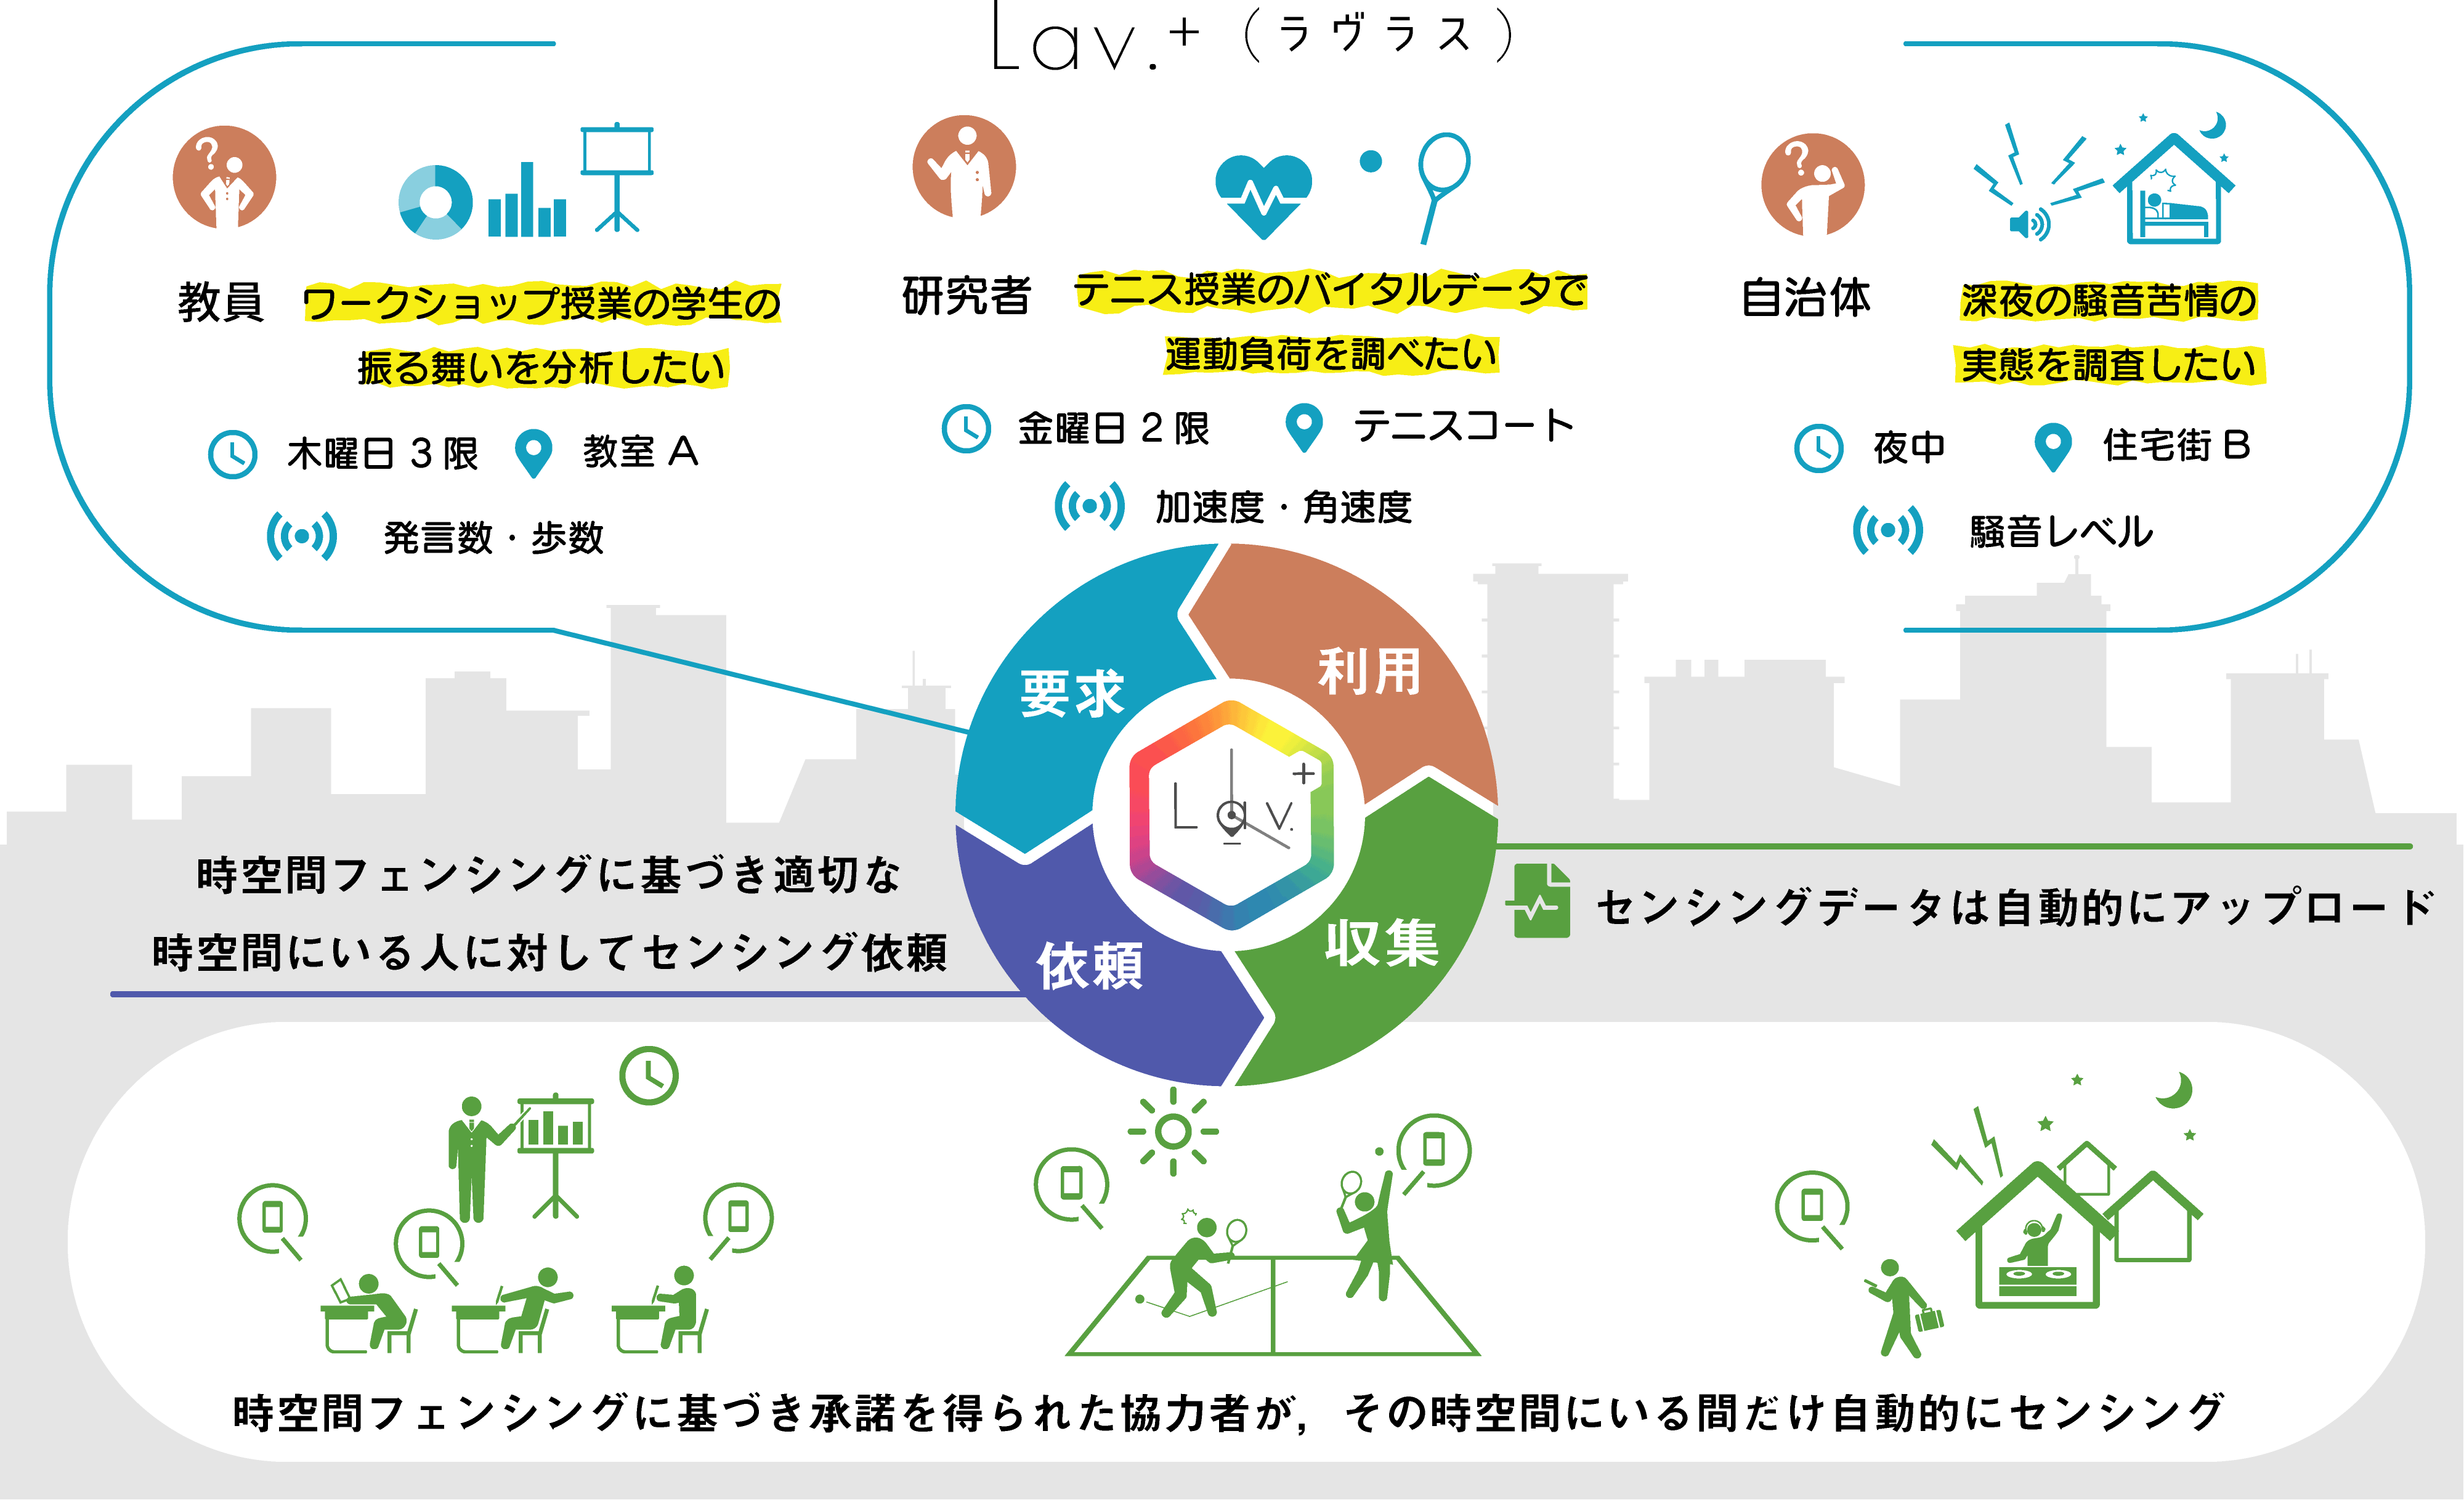
\includegraphics[width=16cm]{img_lavlus.png}
    \caption{ラヴラスの全体像}
    \label{fig:lavlus}
\end{figure}

ラヴラスの全体像を図 \ref{fig:lavlus}に示す.
ラヴラスの一連の流れは「Webアプリでセンシングプロジェクトの定義」,「時空間フェンシング」,「センシング依頼の承諾」,「自動的にセンシング」,「Wi-Fi環境下で自動的にアップロード」,「データ利用」の順で行う.
依頼者はプロジェクト管理Webアプリにて,センシング依頼の内容を細かく定義し,センシングプロジェクトを作成する.
協力者は依頼者の作成したセンシングプロジェクトをダウンロードする.
協力者がセンシングプロジェクトに応じて,\ref{STF}節の定義をもとに時空間フェンシングを行い,協力者が設定された時空間にいる場合のみ通知が送られる.
協力者がセンシング依頼画面に提示された,依頼者とクラウドセンシングの内容に納得し,センシングに協力する場合センシング依頼に承諾する.
協力者がセンシング依頼に承諾し,時空間に進入した場合,バックグラウンドで自動でセンシングが始まる.
センシングが終了し,協力者がWi-Fi下の場合,センサデータをアップロードする.

本プラットフォームは時空間を適切に設定でき,無意識化でセンシングするクラウドセンシングのみ使用できる.
例えば遊園地の経営企業が遊園地の入場者の動向を知るために移動履歴をセンシングしようとしたとする.
その場合,時間は遊園地の開園時間から閉園時間,空間は遊園地内,必要なセンサデータは位置情報と加速度と設定できる.

% (もう一つ例を書きたい,)



% Local Variables: 
% mode: japanese-LaTeX
% TeX-master: "root"
% End: 